\subsection{Method}
\label{subsec:imagelocmethod}

%\begin{comment}
%% Well, this is how we would put two things next to each other if it's ever needed again:
%\begin{figure}
%\begin{floatrow}
%	\ffigbox{
%		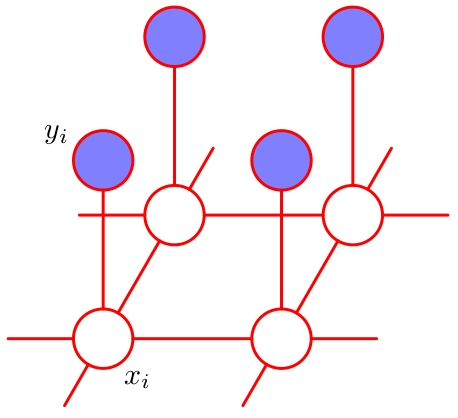
\includegraphics[width=.3\textwidth]{resources/crf}
%	}{
%		\caption{An undirected graph, representing the graph that was used for
%		modeling our Conditional Random Field}
%		\label{fig:crf}
%	}
%	\capbtabbox{%
%		\begin{tabular}{@{\extracolsep{4pt}}l r r r r r r @{}}
%		\hline
%		 & \multicolumn{2}{c}{\emph{SVM only}} & \multicolumn{2}{c}{\emph{Pre-trained}} & \multicolumn{2}{c}{\emph{Direct}} \\
%		 \cline{2-3} \cline{4-5}
%		  & \textbf{Image} & \textbf{Text} & \textbf{Image} & \textbf{Text} \\
%		\textbf{Precision} & 0.269 & 0.979 & 0.241 & 0.979 \\
%		\textbf{Recall} & 0.743 & 0.854 &  0.750 & 0.830 \\
%		\textbf{F-score} & 0.395 & 0.912 & 0.365 & 0.898 \\\hline
%		\end{tabular}
%	}
%	{
%		\caption{scores for image localization with concatenated features}
%		\label{tab:imagelocresults}
%	}
%\end{floatrow}
%\end{figure}
%\end{comment}

The task is to learn a mapping from image patches $y$ to labels $x$. The
observed image patches are HOG features, that are uniformly extracted from the
image. The labels are \emph{text} and \emph{image}. Figure \ref{fig:crf} shows
the structure of the CRF. A label $x_i$ is dependent on the corresponding image
patch $y_i$ and its neighborhood. \footnote{Note, that normally $y$ is used
to denote the labels and $x$ to denote the observed data.  However, following
\cite{lafferty2001conditional, bishop2006pattern}, $y$ was used to denote those
variables that obey the Markov property}.

\begin{wrapfigure}{r}{5cm}
\centering
    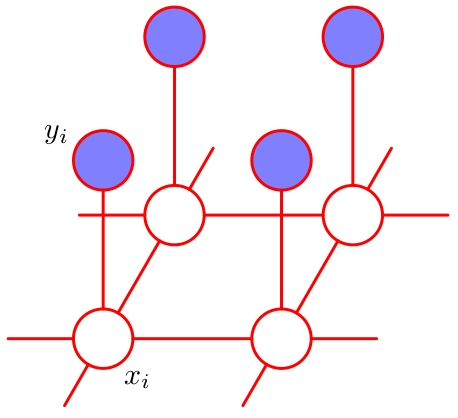
\includegraphics[width=\textwidth]{resources/crf}
    \caption{An undirected graph, representing the graph that was used for
    modeling our Conditional Random Field}
    \label{fig:crf}
\end{wrapfigure}

The energy function can now be defined as follows\cite{bishop2006pattern}:

\begin{align}
E(\mathbf{x}, \mathbf{y}) = h\sum_i x_i - \beta \sum_{\{i, j\}} x_i x_j
- \eta \sum_i x_i y_i
\label{eq:energy}
\end{align}

In \ref{eq:energy}, $\eta$ is a positive constant. The product $\eta \sum_i
x_i y_i$ will then be of a greater number when $x_i$ and $y_i$ are similar.
$\beta$ is another positive constant, which, in combination with the sum of
products $x_i x_j$ should result in higher energy when the neighbouring nodes
$x_j$ have a similar value to $x_i$. Finally $h$ is a constant that can be used
to bias the energy function to either one of the classes, for example when
dealing with an unfair distribution like ours.
%Various implementations of
%Conditional Random Fields might use various types of energy function, but the
%idea is the same.

With the energy function in place a joint distribution can be defined:

\begin{align}
P(x, y) = \frac{1}{Z} exp(-E(x, y))
\end{align}

Where $Z$ is a partition function, used to normalize the probabilities to one.
If we can find the $x$ with the highest probability we would label
the image patches correctly. However, this is not trivial as
looping over all possible solutions is intractable, and a gradient descent
algorithm ends up in a disappointingly low local maximum\cite{bishop2006pattern}.

One of the problems of solving structured SVMs is the reliance on the
weights in the loss function which results in non-convex optimization problem.
This makes them hard to solve. To alleviate this, surrogate loss
functions, which are convex and equivalent to the loss function are
used. Popular surrogate loss constructions are \emph{margin rescaling} and
\emph{slack rescaling}. The convex loss functions can be constructed using a
cutting plane algorithm, which approximates the loss function further until
$\epsilon$ convergence. Using Pystruct \cite{muller2013pystruct} a one slack
structured SVM was trained \cite{joachims2009cutting} to solve the CRFs. The loss
function was the Hamming loss, which counts the amount of patches incorrectly
classified.

Depending on the parameters of the HOG feature extraction the size of the
feature vectors for the image patches can be large. This has significant impact
on the run time of the SVM until convergence. To resolve this a preprocessing
step was implemented in which the feature vector for an image patch is first
assigned a confidence score using a linear SVM. Training this linear SVM is done
in the same manner as the SVM in section \ref{sec:pageclas} was trained on
concatenated feature vectors to classify whole pages. This preprocessing step
can reduce the feature vector to a feature scalar, which saves the required time
to find a solution for the structured SVM.


